\documentclass[AMA,STIX1COL]{WileyNJD-v2}

\articletype{Article Type}%

\received{01 June 2018}
\revised{01 August 2018}
\accepted{01 August 2018}

\raggedbottom
\usepackage{subcaption}
\captionsetup[subfigure]{font=normalsize}

\begin{document}

\title{Room acoustic measurement tool for complex geometry}
%\title{This is the sample article title\protect\thanks{This is an example for title footnote.}}

\author[1]{Robin Gueguen*}

\author[2]{Matthieu Aussal}

%\author[3]{Author Three}

\authormark{ROBIN GUEGUEN \textsc{et al}}


\address[1]{\orgdiv{Institut des Sciences du Calcul et des Donn\'ees}, \orgname{Sorbonne Universit\'e}, \orgaddress{Campus Pierre et Marie Curie - 4 place Jussieu, 75252 Paris Cedex 05 \country{France}}}

\address[2]{\orgdiv{Centre de math\'ematique appliqu\'ees}, \orgname{\'Ecole Polytechnique}, \orgaddress{91128 Palaiseau, \country{France}}}


\corres{\email{gueguen.robin@gmail.com} \\ \email{matthieu.aussal@gmail.com}}

%\presentaddress{This is sample for present address text this is sample for present address text}

\abstract[Summary]{

}

\keywords{acoustic, octree, archeology}

\jnlcitation{\cname{%
\author{R. Gueguen}, and
\author{M. Aussal}, 
} (\cyear{2018}), 
\ctitle{Room acoustic measurement tool for complex geometry}, \cjournal{International Journal for Numerical Methods in Engineering}, \cvol{2018;00:1--6}.}

\maketitle

%\footnotetext{\textbf{Abbreviations:} ANA, anti-nuclear antibodies; APC, antigen-presenting cells; IRF, interferon regulatory factor}


\section{Introduction}\label{sec1}

%Aujourd'hui, les technologies du numériques permettent à la recherche d'explorer des zones jusqu'alors inaccessibles. C'est notamment le cas de l'archéologie architecturale qui utilise de plus en plus la modélisation virtuelle pour découvrir de nouvelles informations. Par ailleurs, la plupart des études se concentrent sur la restitution visuelle d'un bâtiment souvent incomplète. Une étude acoustique peut alors venir renforcer la recherche pour compléter les parties manquantes et aller plus loin dans la compréhension du monde antique. Cela prend du sens lorsqu'on lit les texte traitant d'architecture à l'époque de l'empire Romain \cite{vitruve}. Les architectes concevaient les bâtiments en fonction de la propagation acoustique qu'ils désiraient obtenir. 
%C'est dans le cadre d'un projet de restitution du théâtre antique d'Orange que nous avons donc développé un outil de calcul acoustique adapté à ce type de salle particulière. Effectivement, ce type de bâtiment, une fois virtualisé et maillé présente des centaines de milliers d'éléments ce qui rend les calculs difficiles à réaliser.
%La particularité de ce type de bâtiment est qu'il est très grand (100m de large) que sa géométrie est complexe (avec des surfaces convexes ou concaves) et qu'il est à ciel ouvert. Le modèle numérique a été réalisé avec le logiciel de CAO Blender. Le but de notre outil de calcul acoustique est donc de s'interfacer directement avec ce type d'application. Les calculs doivent pouvoir être effectués sur la plage de fréquences audibles par l'être humain, soit 50 à 15000Hz. Cela rend impossible l'utilisation des méthodes par résolution exactes (éléments finis ou équations intégrales) et, par approximation haute fréquence nous avons opté pour une méthode de lancer de rayons. Celle-ci ne prend en compte que les effets de réflexions et absorptions par la parois en négligeant la diffraction.

Today, digital technologies allow research to explore previously inaccessible areas. This is particularly the case in architectural archaeology, which increasingly uses virtual modelling to discover new information. Moreover, most studies focus on the visual restitution of an often incomplete building. An acoustic study can then come to reinforce the research to complete the missing parts and go further in the understanding of the ancient world. It makes sense when you read texts about architecture during the Roman Empire \cite{vitruve}. Architects designed buildings based on the sound propagation they wanted to achieve. 
It is within the framework of a project of restitution of the ancient theatre of Orange that we developed a tool of acoustic calculation adapted to this type of particular room. Indeed, this type of building, once virtualized and meshed presents hundreds of thousands of elements which makes calculations difficult to carry out. The particularity of this type of building is its significant size (100m wide), its complex geometry (with convex or concave surfaces) and the fact that it is open air. The digital model was created using Blender CAD software. The purpose of our acoustic calculation tool is therefore to interface directly with this kind of application. The calculations must be able to be carried out on the range of frequencies audible by the human being, that is 50 to 15000Hz. This makes it impossible to use exact resolution methods (finite elements or integral equations) and, by high frequency approximation, we opted for a ray tracing method. This one takes only into account the effects of reflections and absorption by the walls while neglecting diffraction.



%\cite{Hirt1974} 
%
%\begin{eqnarray}
%s(nT_{s}) &= &s(t)\times \sum\limits_{n=0}^{N-1} \delta (t-nT_{s}) \xleftrightarrow{\mathrm{DFT}}  S \left(\frac{m}{NT_{s}}\right) \nonumber\\
%&= &\frac{1}{N} \sum\limits_{n=0}^{N-1} \sum\limits_{k=-N/2}^{N/2-1} s_{k} e^{\mathrm{j}2\pi k\Delta fnT_{s}} e^{-j\frac{2\pi}{N}mn}
%\end{eqnarray}




\section{Acoustical energy measurement}\label{sec2}


By modelling a point sound source as a localized pulse in space, the associated energy propagates over time on a spherical surface $\gamma(t)$ such that :

\begin{equation} 
E(t) = E_0 \int_{\gamma(t)} \overrightarrow{I(t)}.\overrightarrow{dS} \qquad \forall t > 0.
\end{equation}

According to the first principle of thermodynamics, if we neglect the effects of losses related to the absorption of the propagation medium, the acoustic energy is preserved over time. Thus, for a point sound source, we have:
\begin{equation} 
\int_{S(t)} \overrightarrow{I(t)}.\overrightarrow{dS} = 1 \qquad \forall t > 0.
\end{equation}

After integration on the spherical surface $S(t)$, we can write the infinitesimal acoustic intensity such as :
\begin{align} 
 \overrightarrow{I}(t) &= \frac{ \overrightarrow{d}(t)}{4\pi d(t)^3} \qquad \forall t > 0 \nonumber, \\
|| \overrightarrow{I}(t) || &= \frac{1}{4\pi d(t)^2} \qquad \forall t > 0,
\end{align}

\begin{figure}
	\centering
	\begin{subfigure}{0.35\textwidth}
		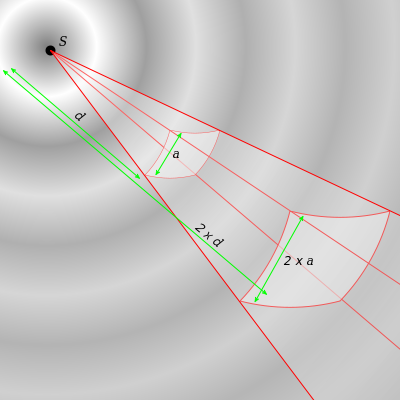
\includegraphics[width=\textwidth]{flux}
		\caption{Representation of the distribution of the energy flow in the propagation of a spherical wave.}
		\label{flux}
	\end{subfigure}
	\begin{subfigure}{0.6\textwidth}
		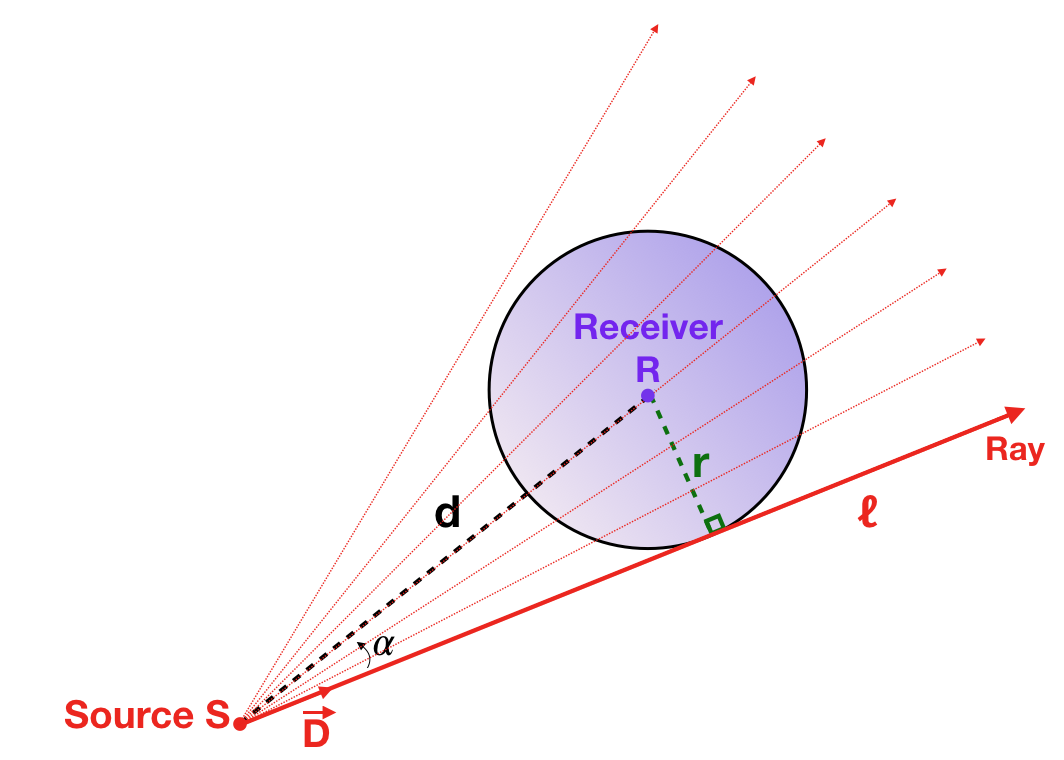
\includegraphics[width=\textwidth]{rays}
		\caption{Representation of rays mesure by a receiver.}
		\label{rays}
	\end{subfigure}	
	\caption{Acoustic emission from a point source.}
\end{figure}

We understand that the intensity decreases as the square of the distance and that a portion of energy considered will therefore be carried by a solid angle (see fig. \ref{flux}). Thus, at a distance $d$ the same amount of energy is distributed over an area of $a^2$ as at a distance of $2d$ over an area of $(2a)^2$. The energy is distributed over an area proportional to the square of the distance. On a portion of $S(t)$ the energy is carried by a solid angle $\Omega_{S}$ such as :
%
\begin{equation} \label{eq_energie}
E_{S}(t) = E_0 \int_{S(t)}  \frac{1}{4\pi  d(t)^2} dS = \frac{E_0}{4\pi}  \Omega_{S}.
\end{equation}
%
This reflects the fact that the energy of a solid angle is constant over time and corresponds to a portion of the initial energy $E_0$. We can then consider the total energy as the sum of energies carried by solid angles such as : 

\begin{equation}
E(t) = \sum_{i=1}^N E_i(t) = \frac{E_0}{4\pi}  \sum_{i=1}^N \Omega_i  \qquad \forall t > 0,
\end{equation}
with  $\Omega_i$ the elementary solid angle : $ \sum_{i=1}^N \Omega_i = 4\pi$. \\

We have chosen to represent each solid angle $ \Omega_i$ by a vector $u_i$, which we will call "ray", and which gives the direction of propagation of the energy $E_i(t)$ over time. Thus, to measure the acoustic energy E(x; t) at a given point in space, we can consider a measuring sphere S(x; r), centred at x and radius r. We can then add the contributions of the n rays that intersect this sphere to calculate the acoustic energy at point x :

\begin{equation}
E(t) = \frac{E_0}{4\pi}\Omega_{S(x,r)} = \frac{E_0}{4\pi}  \sum_{i=1}^n \Omega_i,
\end{equation}

However, to be able to statistically assimilate a set of n rays to a continuous portion of a sphere, it must be ensured that n is large. We use omnidirectional sources, so we can write:
\begin{equation}
	\Omega_i = \frac{4\pi}{N}.
\end{equation}
%
and, by using the formula of a solid angle in a cône, if we consider d, the distance between the source and the receiver sphère S(x; r), we obtain :
\begin{equation}
	\Omega_{S(x,r)} = 4\pi \frac{n}{N} = 2\pi \left(1- \frac{\sqrt{d^2-r^2}}{d}\right).
\end{equation}
%
By fixing n (a number minimum of rays to be caught) and r (the receiver radius) we can get the maximum length of the rays before the measurement become statistically inaccurate :

\begin{equation}
	d_{max} =  \frac{N.r}{2n\sqrt{\frac{N}{n}-1}}.
\end{equation}
%
For large rooms, the total number of rays will be significant (typically N >$10^6$ and n >100) to preserve an accurate measure.

%Example for bibliography citations cite\cite{Taylor1937}, cites\cite{Knupp1999,Kamm2000}

%\begin{figure}[t]
%\centerline{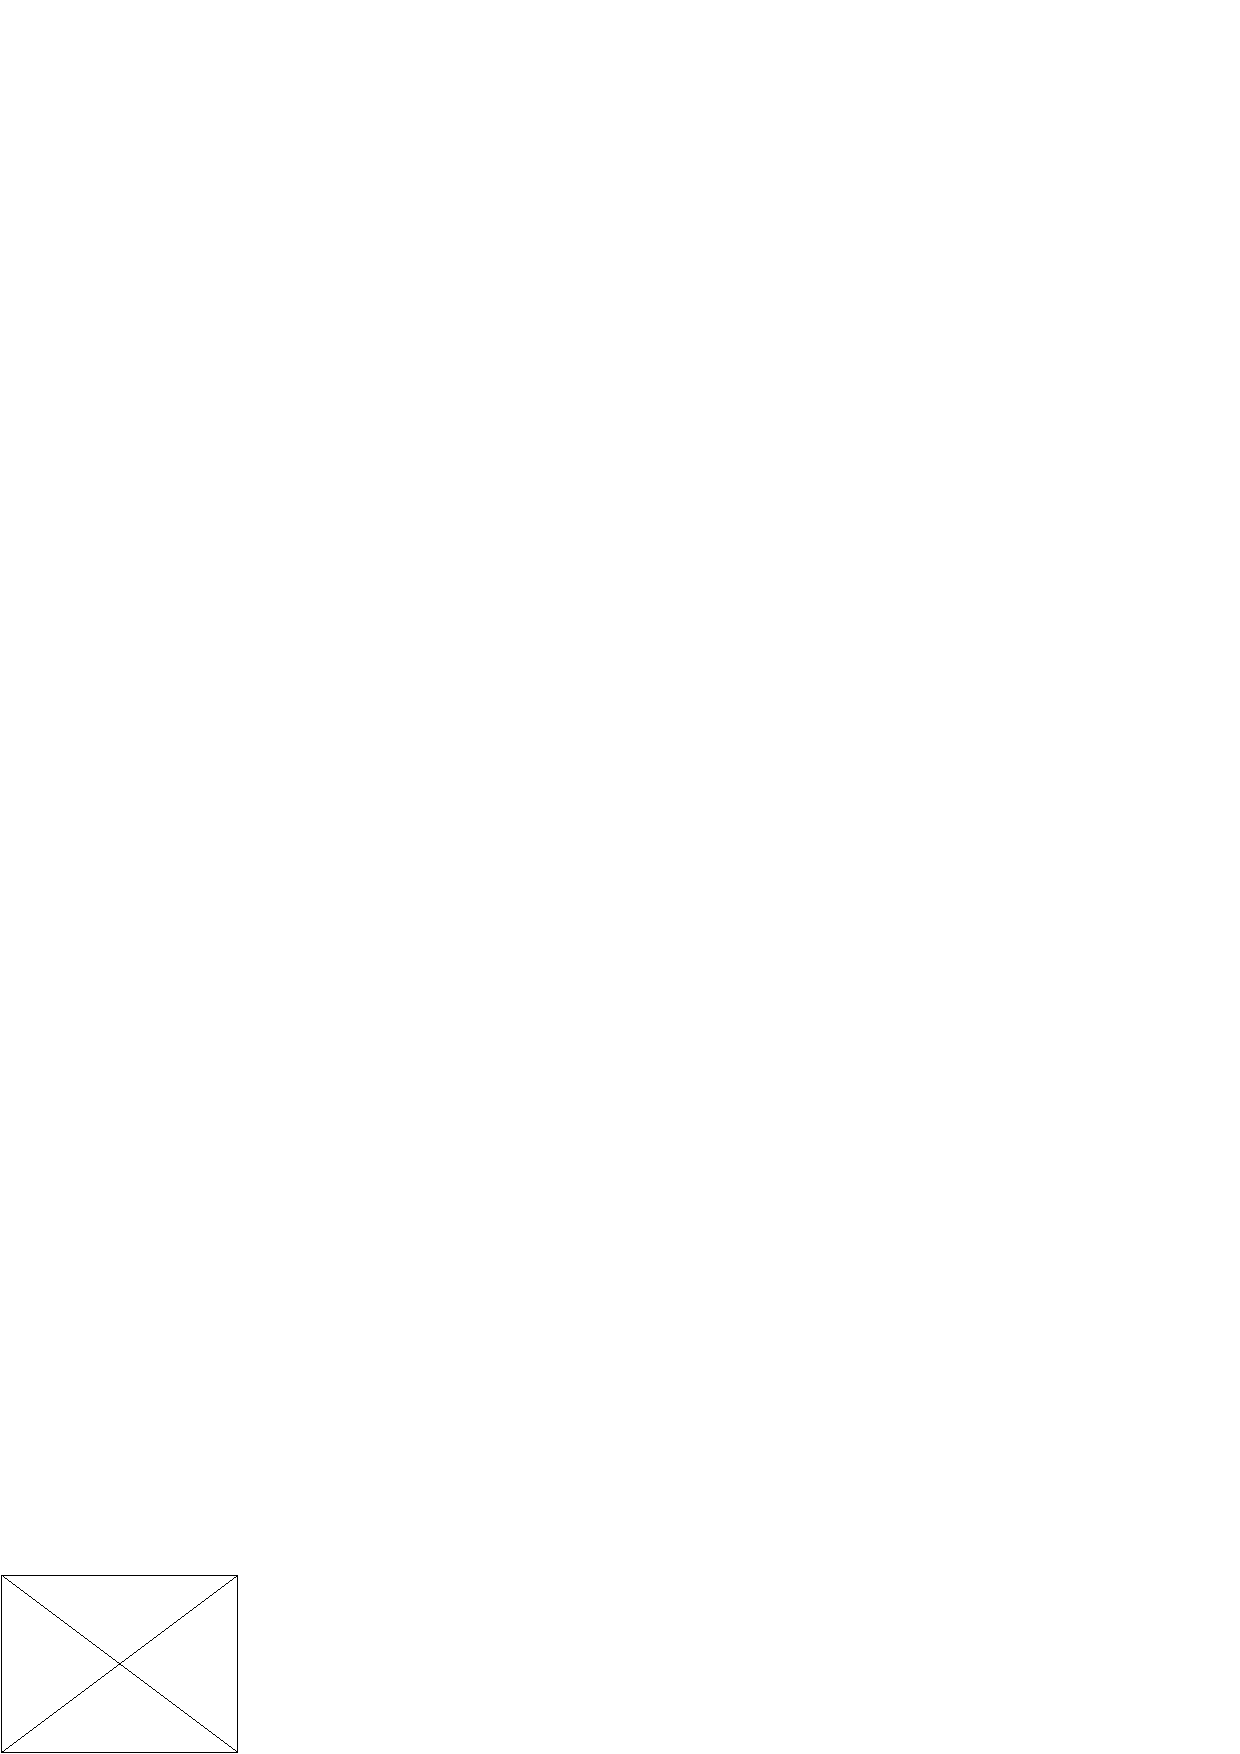
\includegraphics[width=342pt,height=9pc,draft]{empty}}
%\caption{This is the sample figure caption.\label{fig1}}
%\end{figure}



%\subsection{Example for second level head}


\section{Hybride Ray-Tracing / Image-Source methode}\label{sec3}
\subsection{Ray-tracing}

The method developed aims to propagate rays from a point source. A ray is define with the following equation (see fig .\ref{rays}) :
\begin{equation}
\overrightarrow{R}(d) = O + \overrightarrow{D}.d,
\end{equation}
where :
\begin{itemize}
\item $O$ is the origine of the ray,
\item $\overrightarrow{D}$ is the unitary orientation vecteur.
\end{itemize}

To generate $N$ uniform rays, we use a Fibonacci sphere. We note $\Gamma$ the golden ratio such as :
\begin{equation}
\Gamma = \frac{1 + \sqrt{5}}{2}. \\
\end{equation}
%
The spherical coordinates are given by :
\begin{equation}
  \left \{
   \begin{array}{r c l}
\theta &=& \frac{2 \pi \times n}{\Gamma}  \pmod{2\pi},  \\
\phi &=& \arcsin{\left(\frac{2n}{N-1}-1\right)}, 
   \end{array}
   \right .
\end{equation}
%
with : 
\begin{itemize}
\item $N$ : the total number of rays,
\item $n \in[0, 1, 2, \ ... \ ,N-1]$ : the index of the ray.
\end{itemize}
%
Once convert into cartesian coordinates and normalized we can test the intersection with the triangles of the mesh. If a ray intersect a triangle, we can find a point T such as :

\begin{equation} \label{eq_2moller}
T(u,v) = (1-u-v)V_0 + uV_1 + vV_2 = O + D.d,% \ \ \ \footnotemark
\end{equation}
%\citefnt[eq. 2]{moller}
%
with $(u,v)$ the barycentric coordinates such as :
\begin{equation}
   \left \{
   \begin{array}{r c l}
u & \geqslant & -\epsilon,  \\
v & \geqslant & -\epsilon,  \\
(u+v) & \leqslant & 1+\epsilon,
   \end{array}
   \right .
\end{equation}
where $\epsilon = 10^{-5}$ to avoid rounding errors due to machine precision. $d$ is the distance between the point of origin of the ray and the point of intersection. According to Cramer's rule, we can rearrange this equation into the form : :
%
\begin{equation}
	\begin{bmatrix}
 	  -D, & V_1-V_0, & V_2-V_0
	\end{bmatrix}
	\begin{bmatrix}
 	 d \\
	 u \\
	 v
	\end{bmatrix}
	= O-V_0.
	%\ \ \ \footnotemark
\end{equation}
%\citefnt[eq. 4]{moller}
%
Then we get :
\begin{equation}
	\begin{bmatrix}
 	 d \\
	 u \\
	 v
	\end{bmatrix}
	=
	\frac{1}{
	\begin{vmatrix}
 	  -D, & E_1, & E_2
	\end{vmatrix}
	}
	\begin{bmatrix}
 	 	\begin{vmatrix}
 		  T, & E_1, & E_2
		\end{vmatrix} \\
 	 	\begin{vmatrix}
 		  -D, & T, & E_2
		\end{vmatrix} \\
 	 	\begin{vmatrix}
 		  -D, & E_1, & T
		\end{vmatrix}
	\end{bmatrix}	.
	%\footnotemark
\end{equation}
%\citefnt[eq. 5]{moller}
%
with : 
\begin{equation}
   \left \{
   \begin{array}{r c l}
E_1 &=&  V_1-V_0,  \\
E_2 &=&  V_2-V_0,  \\
T &=& O - V_0.
   \end{array}
   \right .
\end{equation}
%
This can be written : 
%
\begin{equation}
	\begin{bmatrix}
 	 d \\
	 u \\
	 v
	\end{bmatrix}
	=
	\frac{1}{
 	  (D \times E_2).E_1
	}
	\begin{bmatrix}
 		  (T \times E_1).E_2
 \\ 
 		  (D \times E_2).T
 \\
 		  (T \times E_1).D
	\end{bmatrix}	.
	%\footnotemark
\end{equation}
%\citefnt[eq. 6]{moller}

The rays can then be reflected on the face as on a mirror to find the new orientation vector :
\begin{equation}
\overrightarrow{r} - \overrightarrow{i} = 2 \times (-\overrightarrow{i}.\overrightarrow{n})\overrightarrow{n}.
\end{equation}
with : 
\begin{itemize}
\item $\overrightarrow{r}$ : the reflected ray,
\item $\overrightarrow{i}$ : the incident ray,
\item $\overrightarrow{n}$ : the normal of the face.
\end{itemize}

\begin{figure}
\centering
	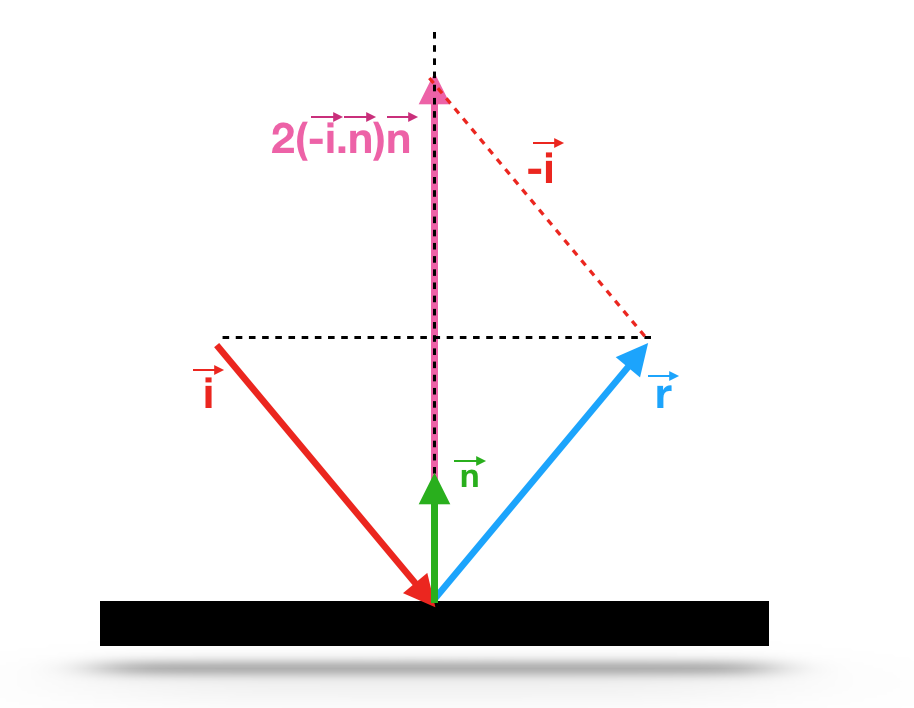
\includegraphics[width=0.4\linewidth]{rayRefl}
	\caption{Calculation of a reflected ray from an incident ray and a normal ray}
	\label{rayRefl}
\end{figure}

Once we know the elements met be each ray we can update their energies. Each triangle carries an an absorption coefficient $\alpha_i$ for every octave band (from 62,5Hz to 8kHz). Moreover, we take into account the atmospheric attenuation. The energy of a ray is :
\begin{equation}
E_{i} =  \frac{E_0}{N} \times \prod_{j=0}^{k}{(1-\alpha_{i,j})} \times e^{-m_i . d_{tot}},
\end{equation}
with : 
\begin{itemize}
\item $E_{i}$ : the energy carried by the ray on the i-th frequency band,
\item $E_{0}$ : the total energy,
\item $k$ : the total number of faces encountered by the rays during its propagation,
\item $j$ : the index of the face encountered par the ray,
\item $m_i$ : the air absorption coefficient in the i-th frequency band (according to the norm ISO-9613),
\item $ d_{tot}$ : the total length of the ray.
\end{itemize}

\subsection{Image-sources}

At each ray bounce, we check if the rays intersect the receiver-sphere. This test includes the following steps :
First we check if the origine point $O$ of the ray is include in the R-center and r-radius receiver :
\begin{equation}
||\overrightarrow{OR}|| \leqslant r,
\end{equation}
%
If not, we check the direction of the ray :
\begin{equation}
\cos{\alpha} \geqslant 0,
\end{equation}
with $\alpha$ the angle between the ray $\overrightarrow{D}$ and $\overrightarrow{OR}$. Then we check if the ray is long enough to reach the receiver :

\begin{equation}
||\overrightarrow{OR}|| \leqslant d,
\end{equation}
%
To finish, we check if the ray intersect the receiver-sphere :

\begin{align}
\sin{\alpha} \times ||\overrightarrow{OR}||  \leqslant r 
\quad \Rightarrow \quad
\alpha  \leqslant \arcsin{\frac{r}{||\overrightarrow{OR}||}}
\end{align}

If the ray does indeed intersect the receiver, an image-source is generated (see fig. \ref{schema_SI}). This is the image of the sound source relative to all the walls encountered by the ray. The image-source $I_S$ is located in space by back-propagation of the ray from its last origin point O :

\begin{equation}
\overrightarrow{I_S O} = \overrightarrow{D}.d_{tot} \qquad \Rightarrow \qquad I_S = O - \overrightarrow{D}.d_{tot},
\end{equation}
where 
\begin{itemize}
\item $\overrightarrow{D}$ is the last unitary orientation vector of the ray,
\item $d_{tot}$ is the total distance travelled by the ray from the original source S to the point O.
\end{itemize}

\begin{figure}
\centering
	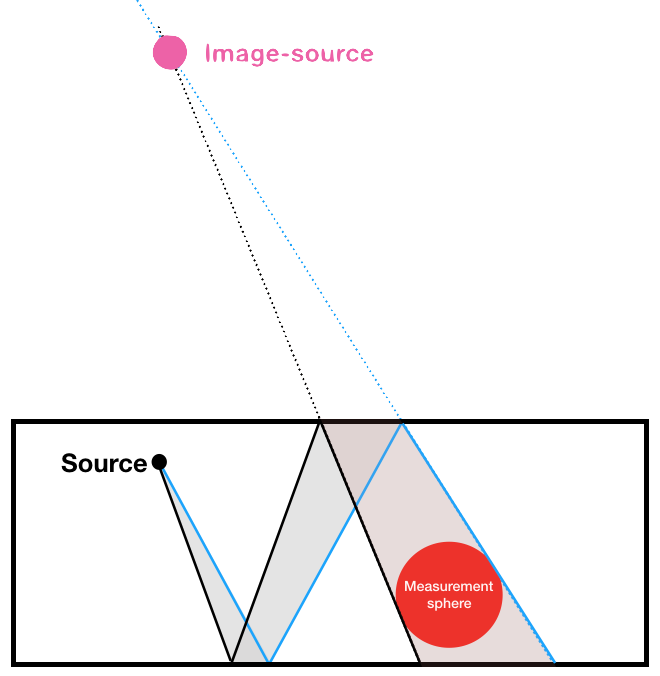
\includegraphics[width=0.3\linewidth]{schema_SI}
	\caption{Sketch of the creation of an image-source by successive reflections of a ray on the walls of a room}
	\label{schema_SI}
\end{figure}

The positions of the image-sources allow to know the time it takes for the signal to arrive to the receiver :

\begin{equation}
t_{I_S} = \frac{||\overrightarrow{I_S O}|| + ||\overrightarrow{OR}||}{v}.
\end{equation}
with $v$ the sound speed in the medium (air : $v=340m/s$). The room impulse response can be generated for each octave band at a certain sampling frequency $f_s$ such as :

\begin{align}
E_{i} =  \sum{E_j},
\end{align}
with the integer part of the product $(t_j \times f_s) = i$ and with : 
\begin{itemize}
\item$E_{i}$ : the energy of the $i^{th}$ sample,
\item$E_j$ and $t_j$ : respectively the energy and travel time of the $j^{th}$ image-source.
\end{itemize}


\section{Algorithm's optimisation}\label{sec4}
\subsection{Presentation}

The algorithm has iteration loops with different complexities. There are three main steps which depend on the number of mesh elements $M$ and the number of rays emitted $N$ :\begin{itemize}
\item the mesh loading,
\item the intersection between rays and faces,
\item the image-sources creation.
\end{itemize}

The mesh loading depends only on the number of elements and is done only once at the beginning of the algorithm. The image-sources creation depends only on the number of rays and is done until the stop threshold is reached. The most critical stage is the intersection of the rays and the faces because each ray has to be tested with each element and the loop is repeated until the stop threshold is reached. The complexity of this operation is quadratic in $O(N\times M)$. For a significant number of mesh elements ($>100~000$ for the Orange theater) and a lot of rays (necessary to make the measurement accurate) the calculation time is very long which makes the tests tedious. To alleviate this problem we have developed a fast algorithm based on a "Divid and conquer" approach based on Octree spatial cutting.

\begin{figure}
\centering
\begin{subfigure}{0.52\textwidth}
	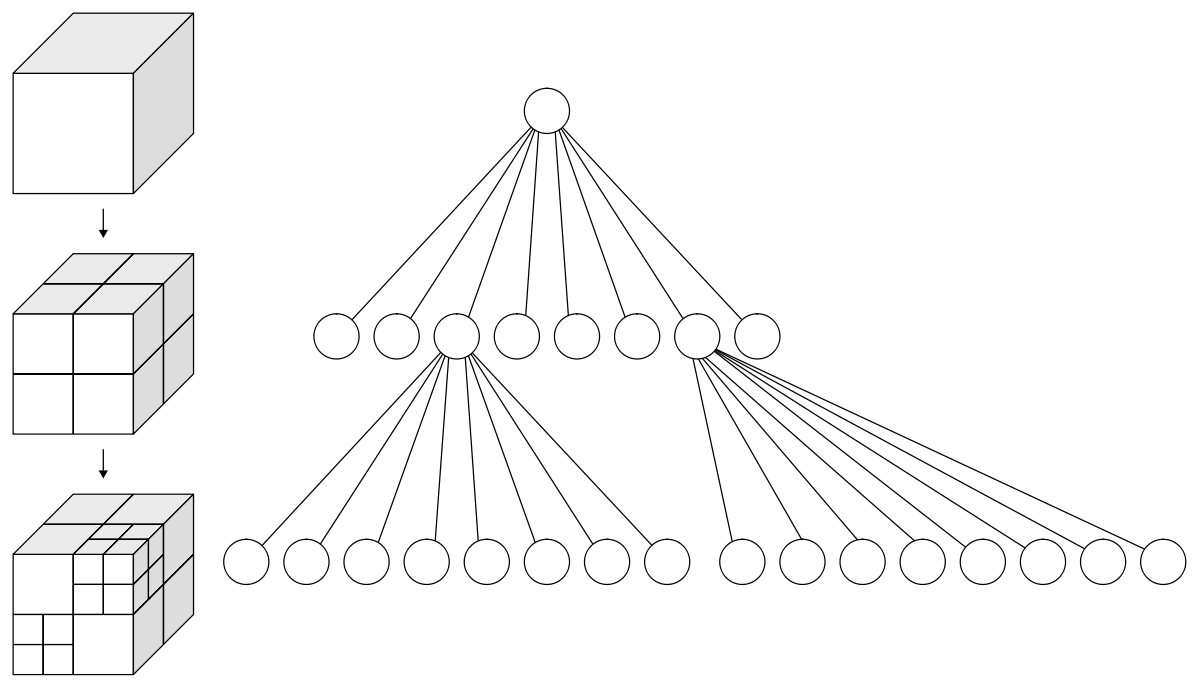
\includegraphics[width=\linewidth]{octree}
	\caption{Illustration of the Octree principle.}
	\label{octree}
	\end{subfigure}
	\begin{subfigure}{0.35\textwidth}
		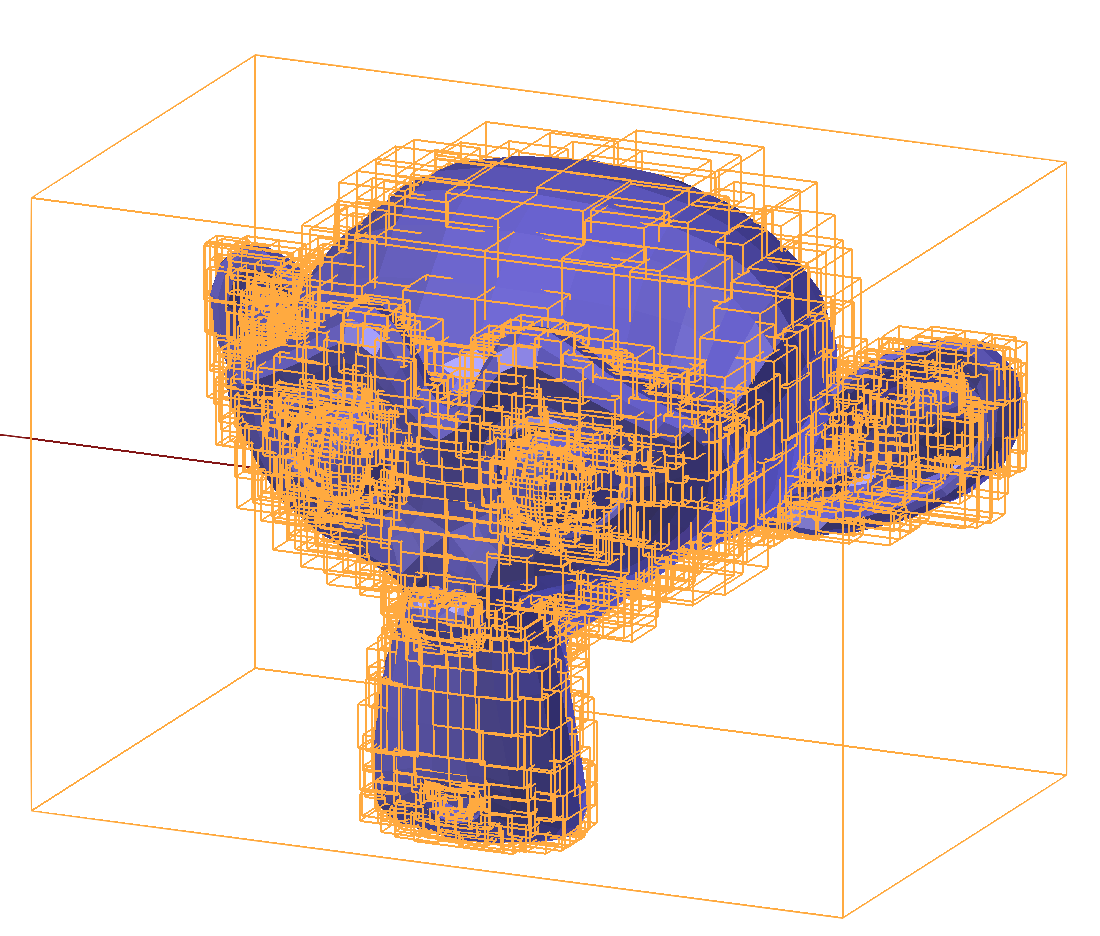
\includegraphics[width=\linewidth]{octreeSuzanne}
		\caption{Octree around an arbitrary mesh}
		\label{octreeSuzanne}
	\end{subfigure}
	\caption{Illustration of an Octree.}
	%\label{octree}
\end{figure}

The general principle consists in creating a cubic box called a "mother box" containing all the mesh elements, i.e. all the triangular faces. This mother box is then subdivided to create eight "daughter boxes" of identical size which themselves will be subdivided into eight daughter boxes, etc. (see fig. \ref{octree}). Recursively, each element contained in a mother box will be stored in the daughter box that contains it. In this way, you descend into the tree structure until you reach a stop condition. Typically, the Octree stops when no more daughter boxes contain more than $n$ items. The boxes are therefore refined in the same way as the mesh (see fig. \ref{octreeSuzanne}) since empty boxes do not generate daughter boxes.

If we name \textit{item} a ray or a triangular face of the mesh and \textit{operation} the storage in a box, we can calculate the number of \textit{operations} a have only one \textit{item} per box. We place ourselves in the case where the \textit{items} are distributed in a uniform way in space. At level-0 all the $N$ \textit{items} are in the root-box. At level-1 we test each daughter box with each \textit{item} and we have $8N$ \textit{operations}. At the next level each daughter box become a mother box and we can apply the same calculation to obtain
\begin{center}
$8\times 8\times \frac{N}{8}$ = $8N$ \textit{operations}.
\end{center}
because each mother box only count $\frac{N}{8}$ \textit{items}. At level-p we will need  
%
\begin{equation} \label{operation}
8^p\frac{N}{8^{p-1}} = 8N \ \textit{operations}.
\end{equation}
%
and the total number of \textit{operations} is $p\times 8N$.

Moreover we said that their is only one \textit{item} per box, so there are as many boxes as there are \textit{items}. We can write :
%
\begin{align}  \label{nbEtage}
8^p &= N \nonumber, \\
p.\ln{8} &= \ln{N} \nonumber, \\
p &= \frac{1}{\ln{8}}\ln{N}.
\end{align}
%
The total number of operation is then :
\begin{equation}
C = p.8N = \frac{8N}{\ln8}\ln{N}.
\end{equation}
%
Within the algorithm, instead of testing all rays with all faces, we test N times one ray with one face. The number of linear operations is :
\begin{equation}
C_{tot} =  \frac{8N}{\ln8}\ln{N} + N.
\end{equation}
which is faster than $N^2$ for $N>>1$.

In practice we will be able to stop the Octree before arriving at only one element per box. Typically, if we stop the Octree at $n$ elements per box the total number of operation become :
\begin{equation}
C_{tot} = \frac{8N}{\ln8}\ln{N} - \frac{\ln n }{\ln8}8N + n^2.
\end{equation}
so $n$ needs to be very small in front of $N$ to preserve the performance.

Note that when the distribution of items is not uniform the demonstration is more complicated but the calculation times remain substantially similar.

\subsection{Implementation}


To store the triangular faces in the box we test if the center of the face belongs to the box. One each center has been store in the leaves of the Octree (i.e the last boxes of the branches) we resize the leaves to embody the whole faces they contains. To test if a ray cross a box we use an algorithm conceived for Axis-Aligned-Bounding-Box. This kind of box can be defined by six plans $\left[ X_{min}, X_{max}, Y_{min}, Y_{max}, Z_{min}, Z_{max} \right] $. If the ray equation is :
\begin{equation}
f(t) = D \times t + O
\end{equation}
with :
\begin{itemize}
\item $D$ : the orientation vector of the whose coordinates are $(D_x ; D_y ; D_z)$,
\item $O$ : the origin point of the ray whose coordinates are $(O_x ; O_y ; O_z)$,
\end{itemize}
we can express the intersection point by this following system :
\begin{align}
X_{min} &= x_0 \times D_x - O_x 	& \Rightarrow 	& &	 x_0 = \frac{X_{min} - O_x}{D_x}, \\
X_{max} &= x_1 \times D_x - O_x 	& \Rightarrow 	& &	x_1 = \frac{X_{max} - O_x}{D_x}, \\
Y_{min} &= y_0 \times D_y - O_y 	& \Rightarrow	& &	y_0 = \frac{Y_{min} - O_y}{D_y}, \\
Y_{max} &= y_1 \times D_y - O_y 	& \Rightarrow	& &	y_1 = \frac{Y_{max} - O_y}{D_y}, \\
Z_{min} &= z_0 \times D_z - O_z	& \Rightarrow 	& &	z_0 = \frac{Z_{min} - O_z}{D_z}, \\
Z_{max} &= z_1 \times D_z - O_z 	& \Rightarrow 	& &	z_1 = \frac{Z_{max} - O_z}{D_z}. 
\end{align}
%
\begin{figure}
\centering
	\begin{subfigure}{0.4\textwidth}
		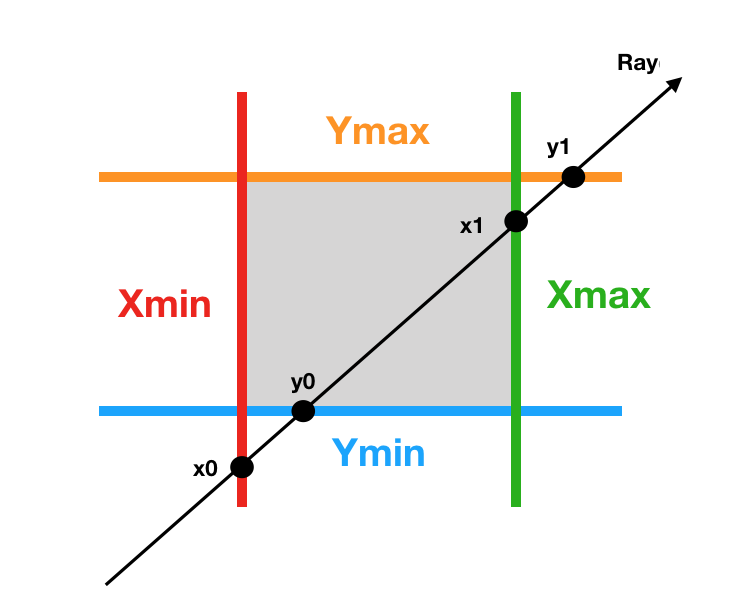
\includegraphics[width=\linewidth]{AABB}
		\caption{Ray/box intersection in 2D}
		\label{AABB}
	\end{subfigure}
	\qquad
	\begin{subfigure}{0.4\textwidth}
		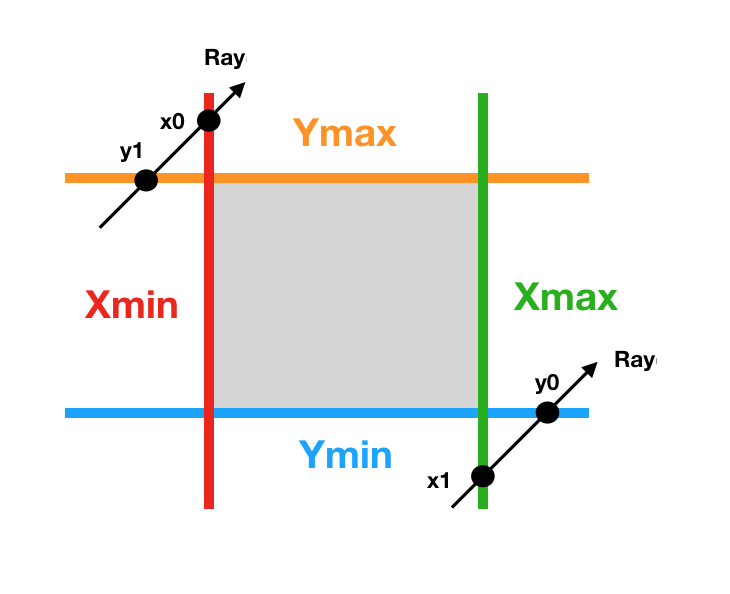
\includegraphics[width=\linewidth]{AABB2}
		\caption{No intersection}
		\label{AABB2}
	\end{subfigure}
	\caption{Illustrations of the ray/box intersection in 2D}
\end{figure}
%
We understand from the figures \ref{AABB} and \ref{AABB2} that we will be able to determine if a ray intersects a box by comparing the coordinates of the points of intersection with the planes. Notably, if $x_0 > y_1$ or $y_0 > x_1$ the radius will not intersect the box (see fig. \ref{AABB2}). Otherwise, the same principle will apply on $z$. There will then be no intersection if $max(x_0 ; y_0) > z_1$ or $ z_0 > min(x_1 ; y_1)$. Note that if the ray is directed in the opposite direction, the $\alpha_0$ and $\alpha_1$ have to be inverted ($\alpha$ corresponding to the coordinates $x,y,z$).


\begin{figure}
\centering
	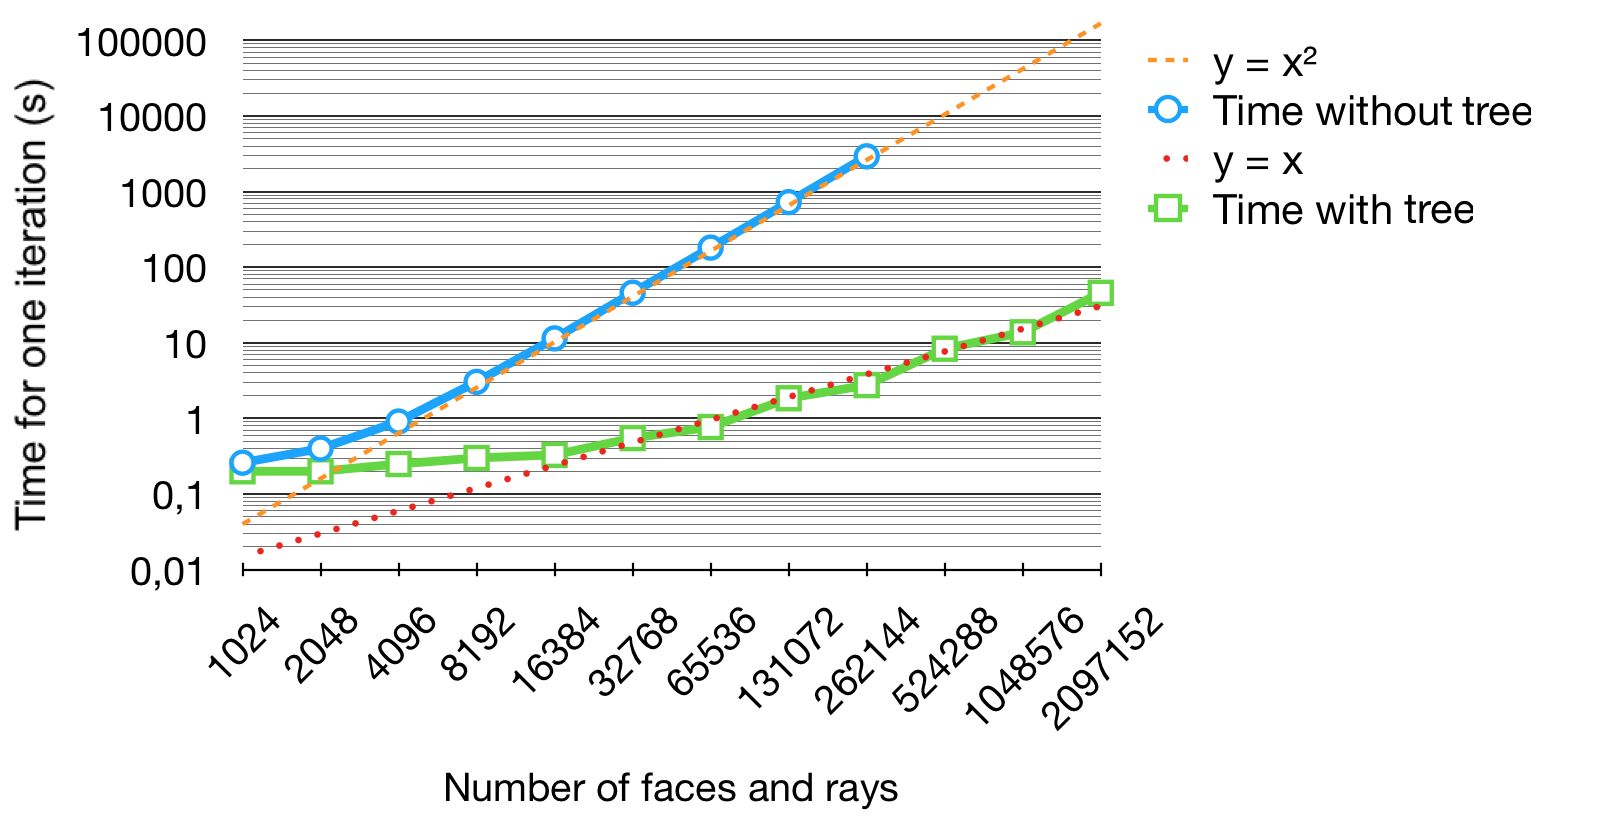
\includegraphics[width=0.8\linewidth]{times}
	\caption{Computation time for one iteration and $N = M$ (log scale)}
	\label{times}
\end{figure}

\begin{table}
\centering
	\begin{tabular}{| c | c | c |}
		\hline
		Number of faces and rays & Time \textbf{without} Octree (s) & Time \textbf{with} Octree (s)\\
		  \hline
		  \hline
		   $2^{10}$ (=1~024) & 0,26 &	0,2 \\
		   \hline
		$2^{11}$ (=2~048)  & 0,4	& 0,2 \\
		   \hline
		$2^{12}$ (=4~096) & 0,91	& 0,25\\
		   \hline
		$2^{13}$ (=8~192) & 3,05 &	0,3\\
		   \hline
		$2^{14}$ (=16~384) & 11,44	&0,33\\
		   \hline
		$2^{15}$ (=32~768) & 46,02	&0,55 \\
		     \hline
		    $2^{16}$ (=65~536) & 181,61	& 0,77\\
		   \hline
		$2^{17}$ (=131~072) & 725,17	& 1,85\\
		\hline
		$2^{18}$ (=262~144) & 2927,9 & 2,76 \\
		\hline
		$2^{19}$ (=524~288) & X & 8,36 \\
		\hline
		$2^{20}$ (=1~048~576) & X & 13,78 \\
		\hline
		%$2^{21}$ (=2~097~152) & X & 45,83 \\
		%\hline
	 \end{tabular}
	\caption{Computation time for one iteration and $N = M$}
	\label{tabComplexite}
\end{table}

As we can see in the figure \ref{times} the complexity of the algorithm is almost linear by using the Octree method. This allows to treat large meshes with millions of rays by maintaining a low computation time. In particular, we can see in the table \ref{tabComplexite} that for 250~000 rays and faces the computation time is divided by 1000. 

\section{Validation}\label{sec5}

In order to validate our approach and our method we compare the experimental results with theoretical results. 

\subsection{Quadratic decrease}
First, to validate the quadratic decrease of the energy we observe the room impulse response of a cubic room whose all walls are 100\% absorbant except the walls on the x-axis. This particular room reflect a free space simulation where the distance between the source and the receiver is regularly increased. Furthermore, since the rays spread on the x-axis and -x-axis and return in phase, the number of rays received is twice the number of rays in free space.
%
\begin{figure}
\centering
	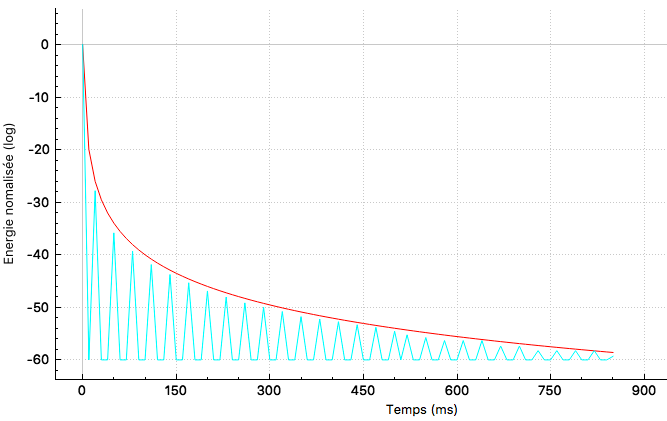
\includegraphics[width=0.6\linewidth]{test1}
	\caption{RIR for 3 millions of rays (blue) sampled at 100Hz and $f(x)=\frac{2}{x^2}$ (red)}
	\label{test1}
\end{figure}
%
The room impulse response follow the $f(x)=\frac{2}{x^2}$ which is the expected behavior. In free space, the number of rays collected expresse the surfaces ratio and the quadratic decrease :
\begin{equation}
\frac{n}{N} = \frac{\int_s dS}{\int_{\sigma} dS} = \frac{\pi r^2}{4\pi d^2},
\end{equation}
avec :
\begin{itemize}
\item$n$ : the number of rays collected,
\item$N$ : the total number of rays,
\item$s$ : the constant surface of the receiver collecting rays (disk),
\item$\sigma$ : the emission sphere surface,
\item$r$ : the constant radius of the receiver,
\item$d$ : the emission sphere radius (i.e the distance between the source and the receiver).
\end{itemize}

\subsection {Energy conservation}
The second test allows to simulate the conservation of the energy. We use a 100\% reflecting sphere (2m radius) pretty well refined (300~000 faces) and position the source and the receiver in the center. So, at each iteration all the rays refocus in the center of the sphere and then are captured by the receiver.
\begin{figure}
\centering
	\begin{subfigure}{0.45\textwidth}
		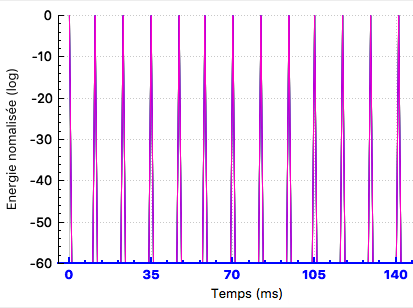
\includegraphics[width=\linewidth]{test2RIR}
		\caption{RIR for a 100\% reflecting sphere - 12 iterations}
		\label{test2RIR}
	\end{subfigure}
	\quad
	\begin{subfigure}{0.38\textwidth}
		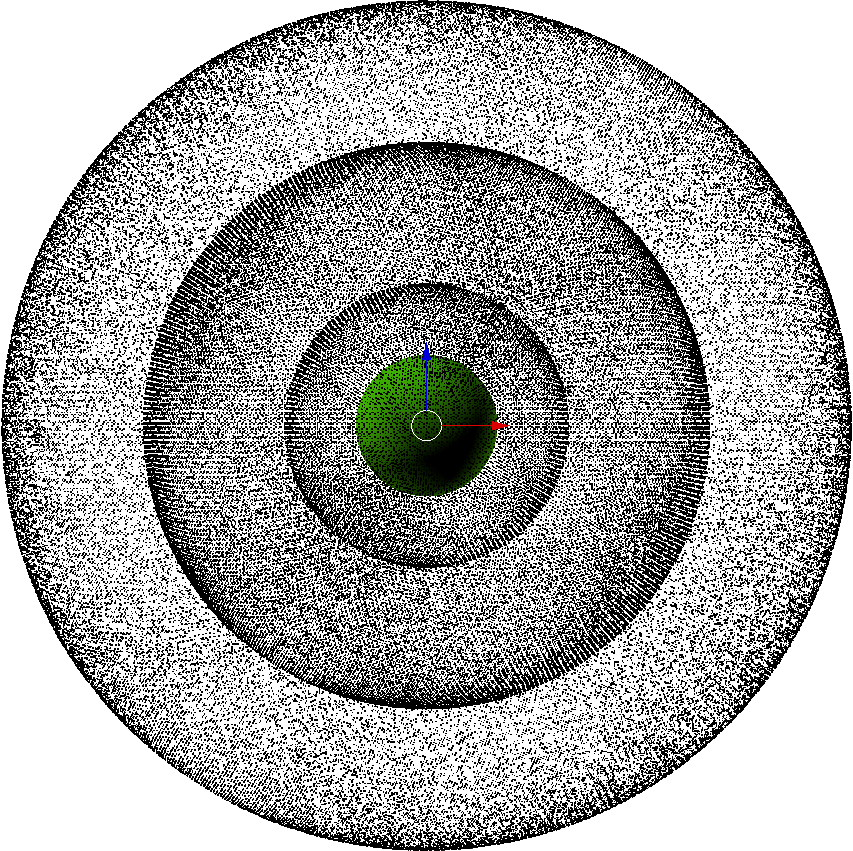
\includegraphics[width=\linewidth]{test2SI}
		\caption{Position of the images-sources - 4 iterations}
		\label{test2SI}
	\end{subfigure}
	\caption{100\% reflecting sphere}
\end{figure}
%
We observe the expected result as the room impulse response is a Dirac comb (see fig. \ref{test2RIR}) and the image-sources are positioned on spheres whose the radius doubles at each iteration (see fig. \ref{test2SI}).
%
\begin{figure}
\centering
	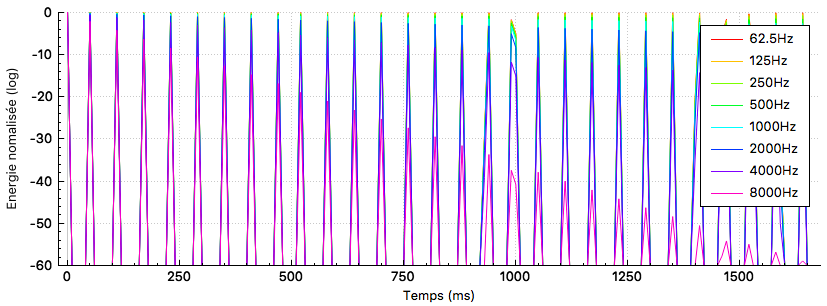
\includegraphics[width=0.6\linewidth]{test2absair}
	\caption{RIR for a 100\% reflecting sphere with air absorption - 30 iterations}
	\label{test2absair}
\end{figure}
%
By adding the air absorption we can observe that the highest frequencies decrease faster than the lowest which reflect the nature behavior.

\subsection{Shoe box case}
To finalize the validation algorithm we compare the results of a shoe box type room with an analytic computation. The image-sources can be positioned in space with the following formula :
\begin{align}
P_{is} = i \times D + P_s \times (-1)^i,
\end{align}
with : 
\begin{itemize}
\item$i \in (-n, n)$ and $n \in \mathbb{N}$,
\item$P_{is}$ : the image-source position coordinate on X, Y or Z,
\item$P_s$ : the source position coordinate on X, Y or Z,
\item$D$ : the room dimension on X, Y or Z.
\end{itemize}
The energy of each image-source is $\frac{1}{d^2}$ where $d$ is the distance between the image-source avec the receiver. If we compare the position of these theoretical image-sources with the image-sources obtained with the algorithm we gat the exact same result to the float precision ($10^{-6}m$). Concerning the energy, we compare two kind of errors : the relative error such as :
\begin{align}
\epsilon_{rel} = \frac{|E_{exp}-E_{theo}|}{E_{theo}}.
\end{align}
and the infinity norm error with express the fact that the further away the image-source is from the receiver the less important the error will be for the final result.
\begin{align}
\epsilon_{\infty} = \frac{|E_{exp}-E_{theo}|}{\max(E_{theo})}.
\end{align}
We can also add some absorption coefficient on the walls and take into account the air absorption. We can see in the figure \ref{test3_8} that the relative error of the energy image-source per image-source remains always below 5\% and in the figure \ref{test3_9} that the infinity norm error is below $0,3\%$ for all frequencies.

\begin{figure}
\centering
	\begin{subfigure}{0.49\textwidth}
		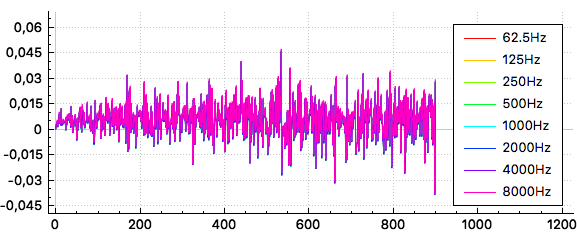
\includegraphics[width=\linewidth]{test3_8}
		\caption{Relative error}
		\label{test3_8}
	\end{subfigure}
	\begin{subfigure}{0.49\textwidth}
		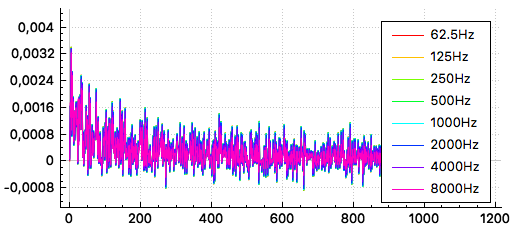
\includegraphics[width=\linewidth]{test3_9}
		\caption{Infinity norm error}
		\label{test3_9}
	\end{subfigure}
	\caption{Error for each image-sources with walls and air absorption - 1~000~000 rays}
\end{figure}


\section{Developed softwares }\label{sec6}

The room acoustic tool is available in two forms. 

\subsection{Matlab library}
First a Matlab library ... \\

\subsection{Blender add-on}
In a second hand the tool is also available as a Blender add-on. The user can work on the CAD software to model the room under test, positioning the sources and the receiver and assign materials to the walls. By clicking on the "Run" button, the mesh is exported, the materials are linked to eight absorption coefficients (extracted from a data base) and the acoustic calculation tool is launched. This is an executable C++ complied software which treats information form Blender and generates the room impulse response. The communication between the CAD and the executable is done thanks to an .obj file, so using Blender is not necessary. Different options allow to analyse the results by reimporting rays or image-sources on the CAD software. It is also possible to listen an audio file convolved to to RIR to listen the reverberate sound.


%\begin{figure}
%	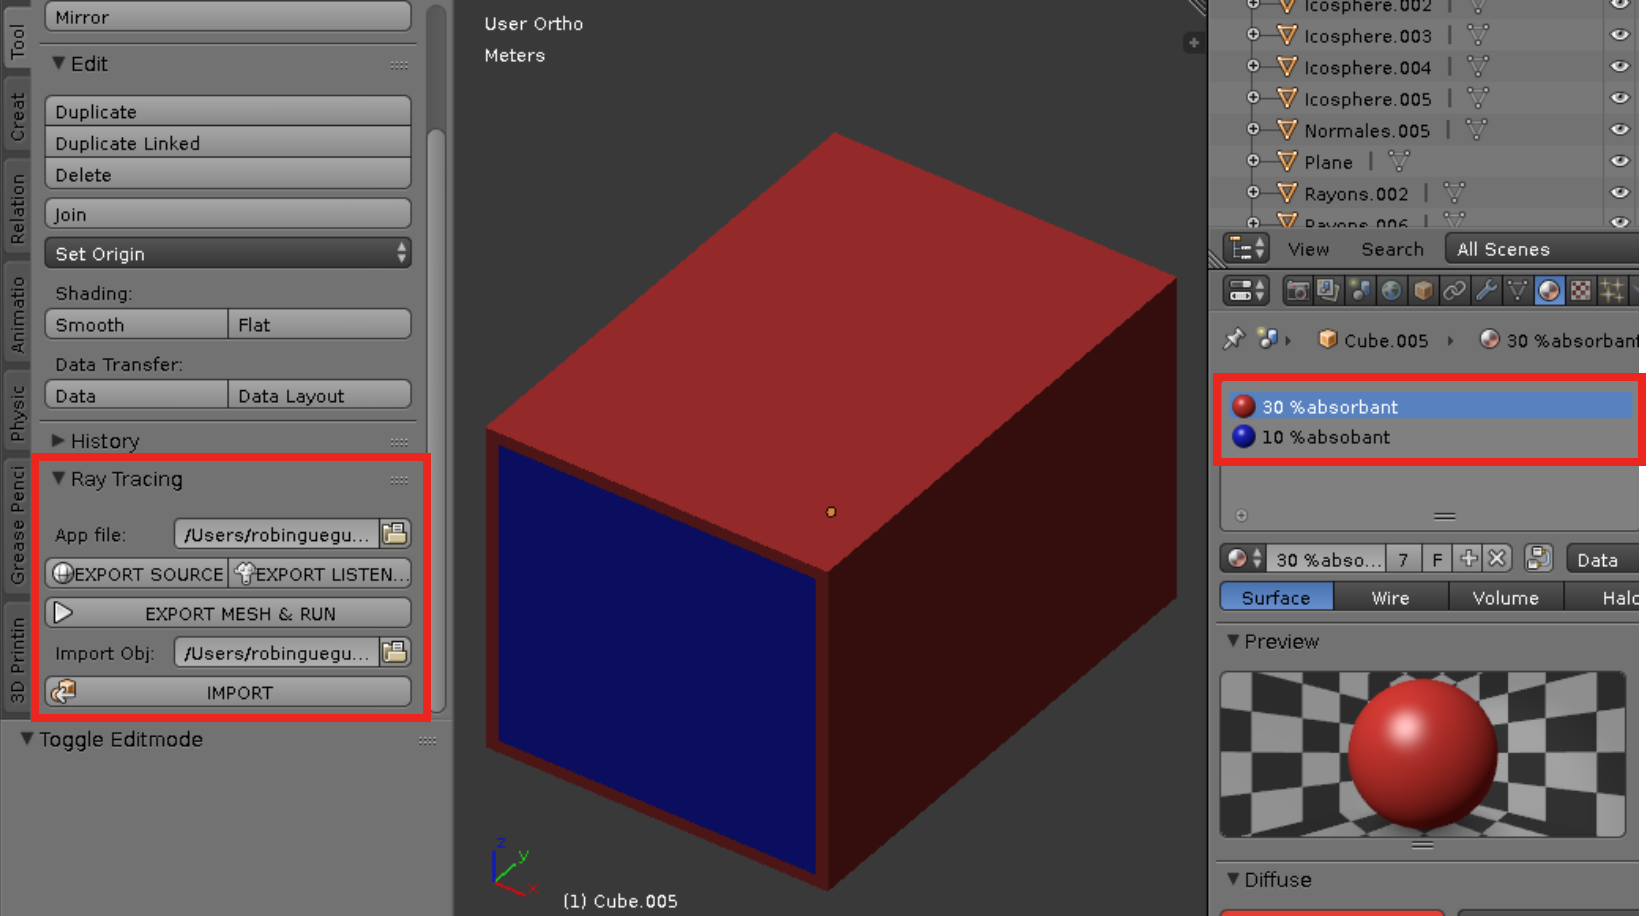
\includegraphics[width=\linewidth]{add-on}
%	\caption{Add-on Blender}
%\end{figure}

\begin{figure}
\centering
	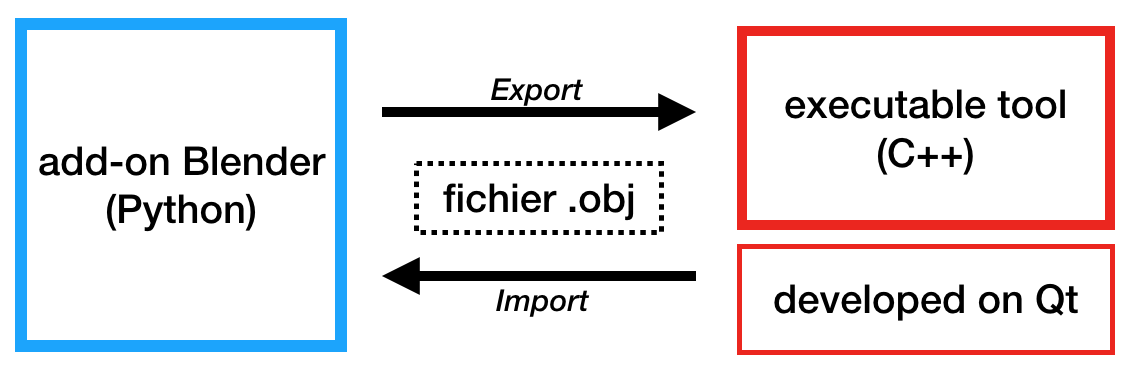
\includegraphics[width=0.7\linewidth]{software}
	\caption{Software architecture}
\end{figure}



\section{Application to the antic theatre of Orange}\label{sec7}

The acoustic simulation can be done on the antic theater fo Orange. Because it is an open room the software automatically add a 100\% absorbant box around the building and we can calculate the image-sources and the RIR for different configuration of the theatre or different materials. Indeed, archeologists want to explore some architecture hypothesis from missing part of the theatre. A acoustical analysis can allow to understand better the influence of the position in the bleachers, the shape of the roof, the material of the \textit{orchestra} for exemple.With a 600~000 faces theatre (i.e including decoration elements of the stage wall) RIR at $RT_{60} $is generated in 20 minutes for one million rays (see fig. \ref{rir}). Each iteration is done in 25s so it really depends on the materials chosen. We can note that the more details of the mesh are refined the more we can simulate diffraction effect. Indeed, in high frequency, small detail elements will be able to reflect the rays in different directions which can resemble diffraction effects.

\begin{figure}
\centering
	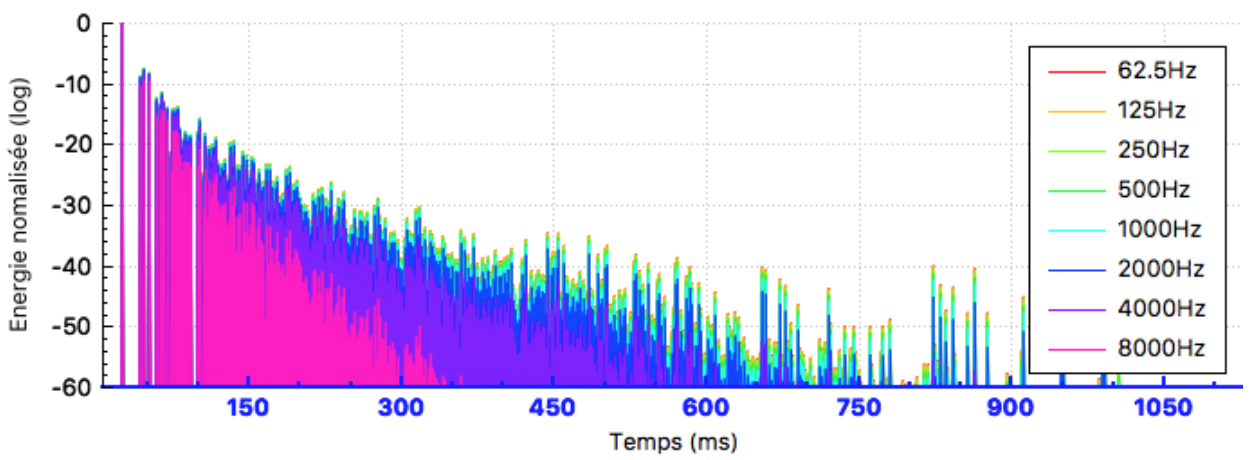
\includegraphics[width=0.7\linewidth]{rir}
	\caption{Room impulse response of the antic theater of Orange}
\end{figure}

\begin{figure}
\centering
	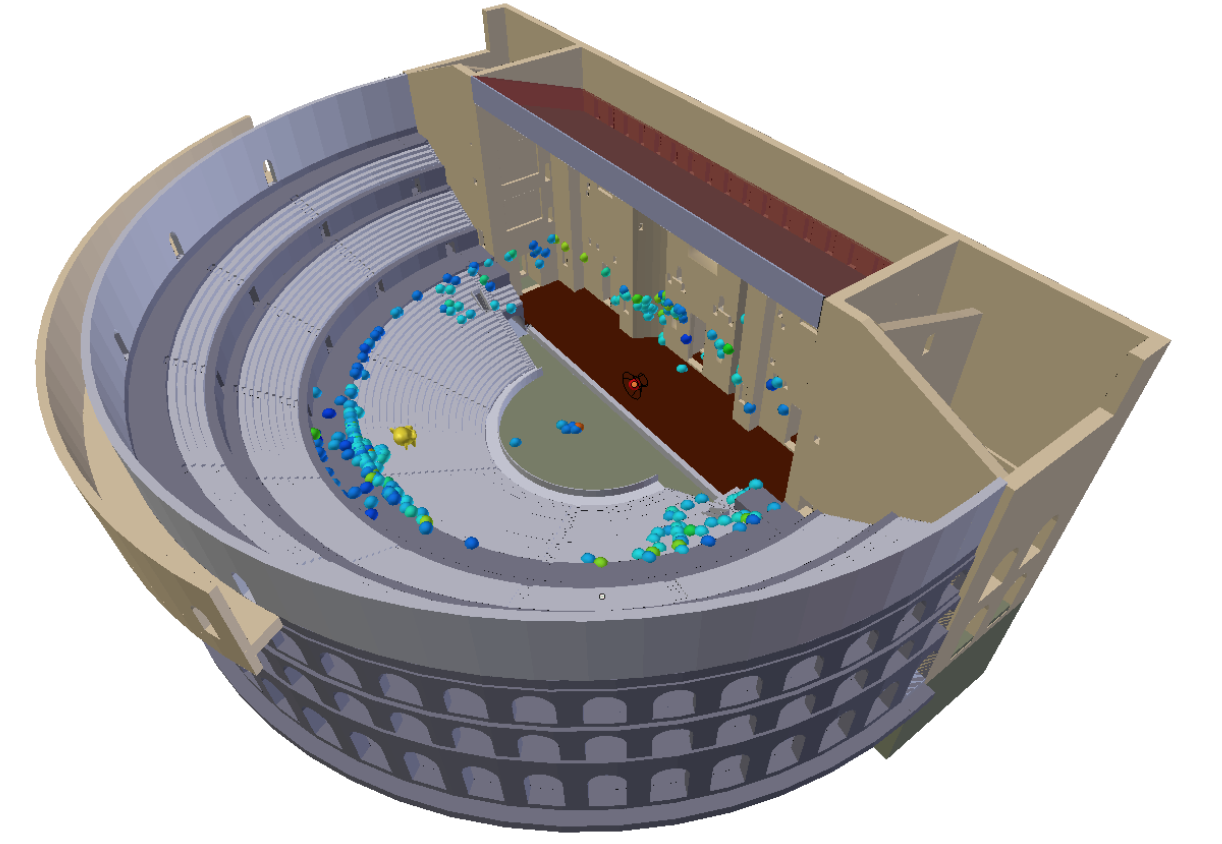
\includegraphics[width=0.7\linewidth]{theatre}
	\caption{Images-sources projected on the theatre of Orange}
\end{figure}


\section{Conclusions}

We presented the problems raised by an acoustic study of an ancient monument. The complex geometry of this type of building and their colossal size requires the use of approximate calculation methods. Thus, by simulating the reflections and absorptions of the walls, it is possible to study the reverberation of a room. Despite the inevitable approximations of the model, we have proved that the laws of physics are respected. A fast algorithm has been implemented to allow users to easily and quickly test their architectural assumptions. Thus, the calculation time becomes little sensitive to the number of mesh elements, which is often limiting in this type of study. The algorithm developed allows the study of the temporal graph of reverberation of the building as well as the position in space of the various sound reflections.

However, there are many opportunities for improvement that remain under consideration for this type of software tool. Firstly, the sound signal could be heard in three dimensions thanks to binaural filters. These allow through an audio headset to transmit a different signal to each of the two ears in order to give the illusion of space and depth. This can be achieved by calculating the positioning of image sources in space. Steering control could then be performed using the keyboard or a headset with "Head Tracker". Secondly, in a context where virtual reality is becoming more and more important in today's applications, we could consider moving the listener in real time and thus allow a complete virtual tour of the building.

From the point of view of the analysis results, there are many possible improvements at the graphical level. That raises some questions. How to view acoustic calculation results? What information is essential for an archaeologist wishing to study the acoustics of a monument? Similarly, is it essential to add diffraction effects to the model? If so, what is the best method? Could certain acoustic behaviours be treated locally and then inserted into the model by ray throwing? 

Finally, it would also be interesting to use sources whose directivity is not uniform. This would be more representative of the real cases and in particular of the use made in Orange at the origin of the theatre. The sounds were then emitted by musical instruments or by the human voice possibly amplified by a mask.

\section*{Acknowledgments}


\subsection*{Author contributions}
 

\subsection*{Financial disclosure}

None reported.

\subsection*{Conflict of interest}

The authors declare no potential conflict of interests.


\section*{Supporting information}

%The following supporting information is available as part of the online article:
%
%\noindent
%\textbf{Figure S1.}
%{500{\uns}hPa geopotential anomalies for GC2C calculated against the ERA Interim reanalysis. The period is 1989--2008.}
%
%\noindent
%\textbf{Figure S2.}
%{The SST anomalies for GC2C calculated against the observations (OIsst).}


\appendix

\section{Section title of first appendix\label{app1}}

%Use \verb+\begin{verbatim}...\end{verbatim}+ for program codes without math. Use \verb+\begin{alltt}...\end{alltt}+ for program codes with math. Based on the text provided inside the optional argument of \verb+\begin{code}[Psecode|Listing|Box|Code|+\hfill\break \verb+Specification|Procedure|Sourcecode|Program]...+ \verb+\end{code}+ tag corresponding boxed like floats are generated. Also note that \verb+\begin{code}[Code|Listing]...+ \verb+\end{code}+ tag with either Code or Listing text as optional argument text are set with computer modern typewriter font.  All other code environments are set with normal text font. Refer below example:
%
%\begin{lstlisting}[caption={Descriptive Caption Text},label=DescriptiveLabel]
%for i:=maxint to 0 do
%begin
%{ do nothing }
%end;
%Write('Case insensitive ');
%WritE('Pascal keywords.');
%\end{lstlisting}
%
%
%
%\subsection{Subsection title of first appendix\label{app1.1a}}
%
%\noindent\textbf{Unnumbered figure}
%
%
%\begin{center}
%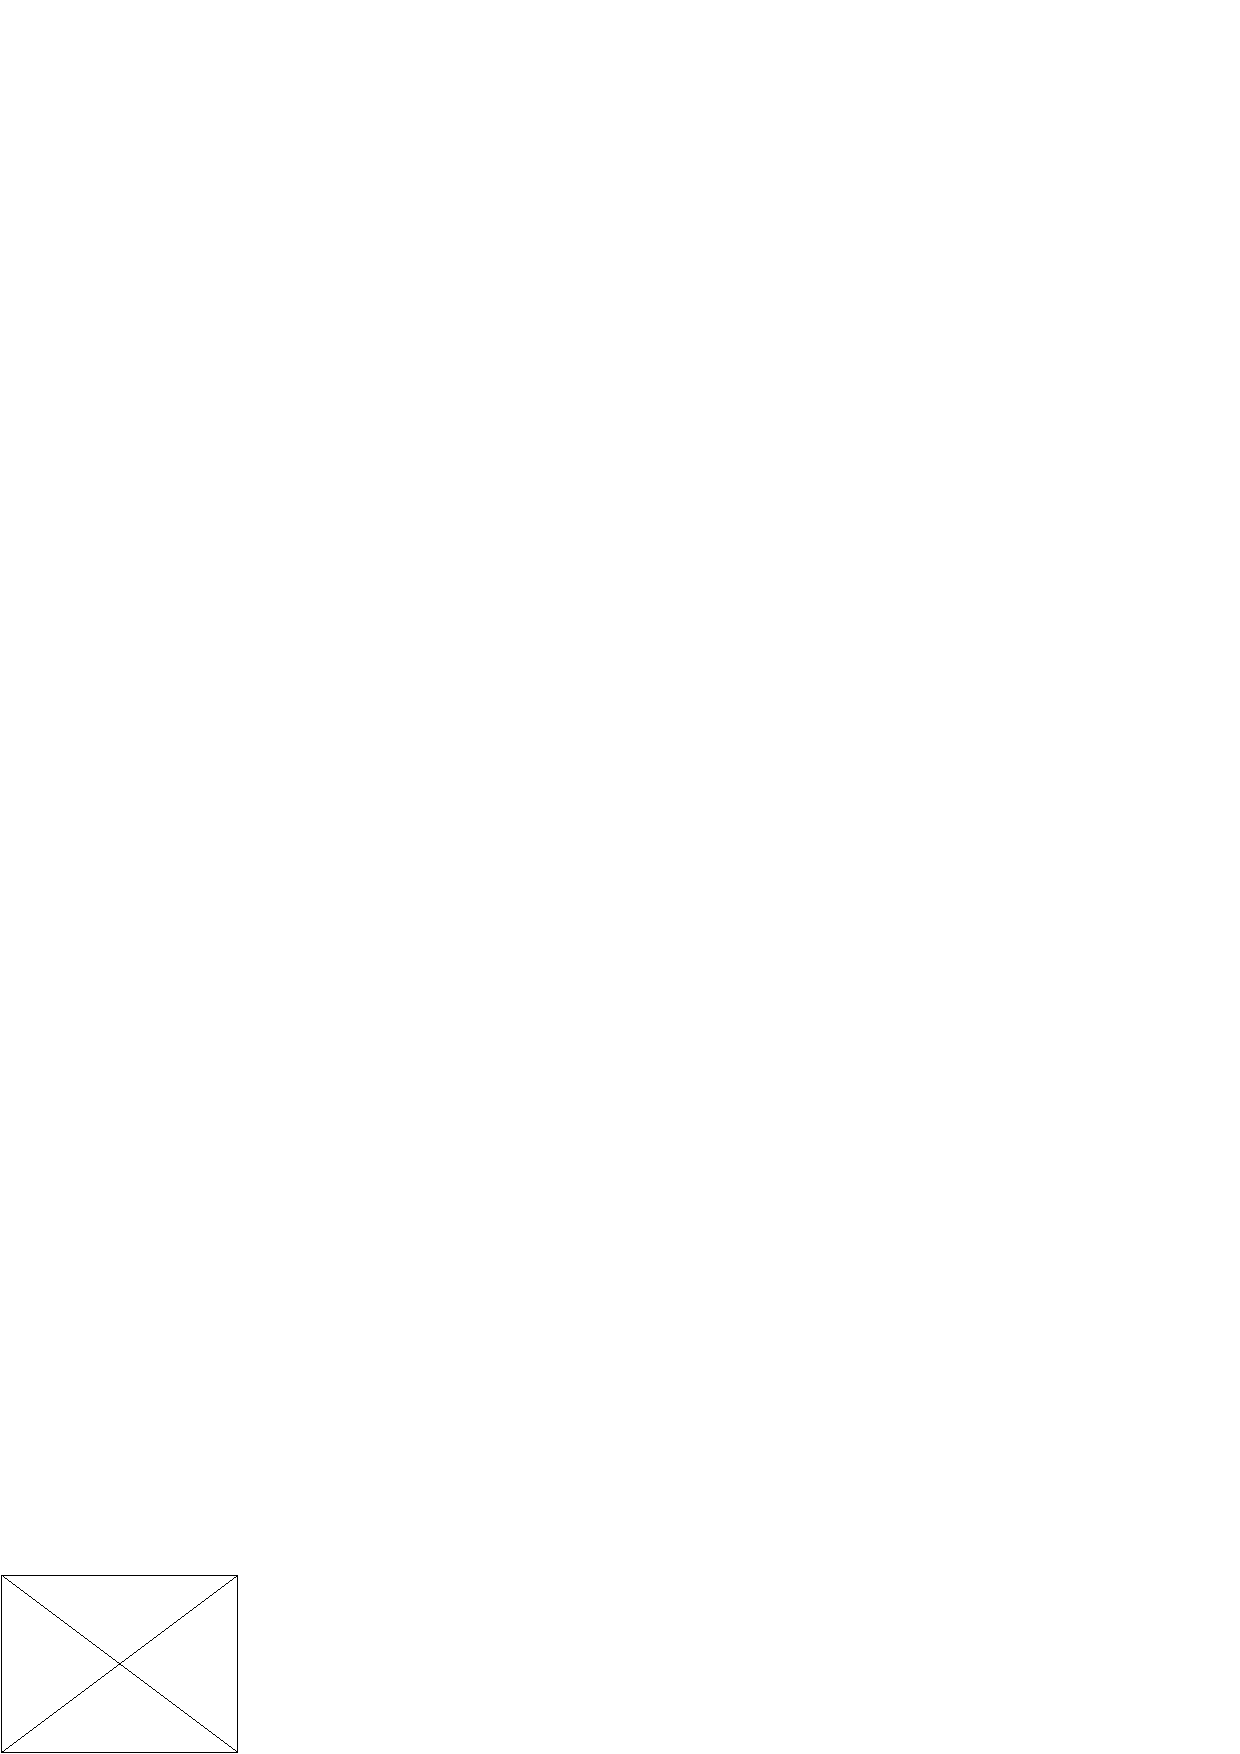
\includegraphics[width=7pc,height=8pc,draft]{empty}
%\end{center}
%
%
%%== Figure 4 ==
%%% Example for figure inside appendix
%\begin{figure}[t]
%\centerline{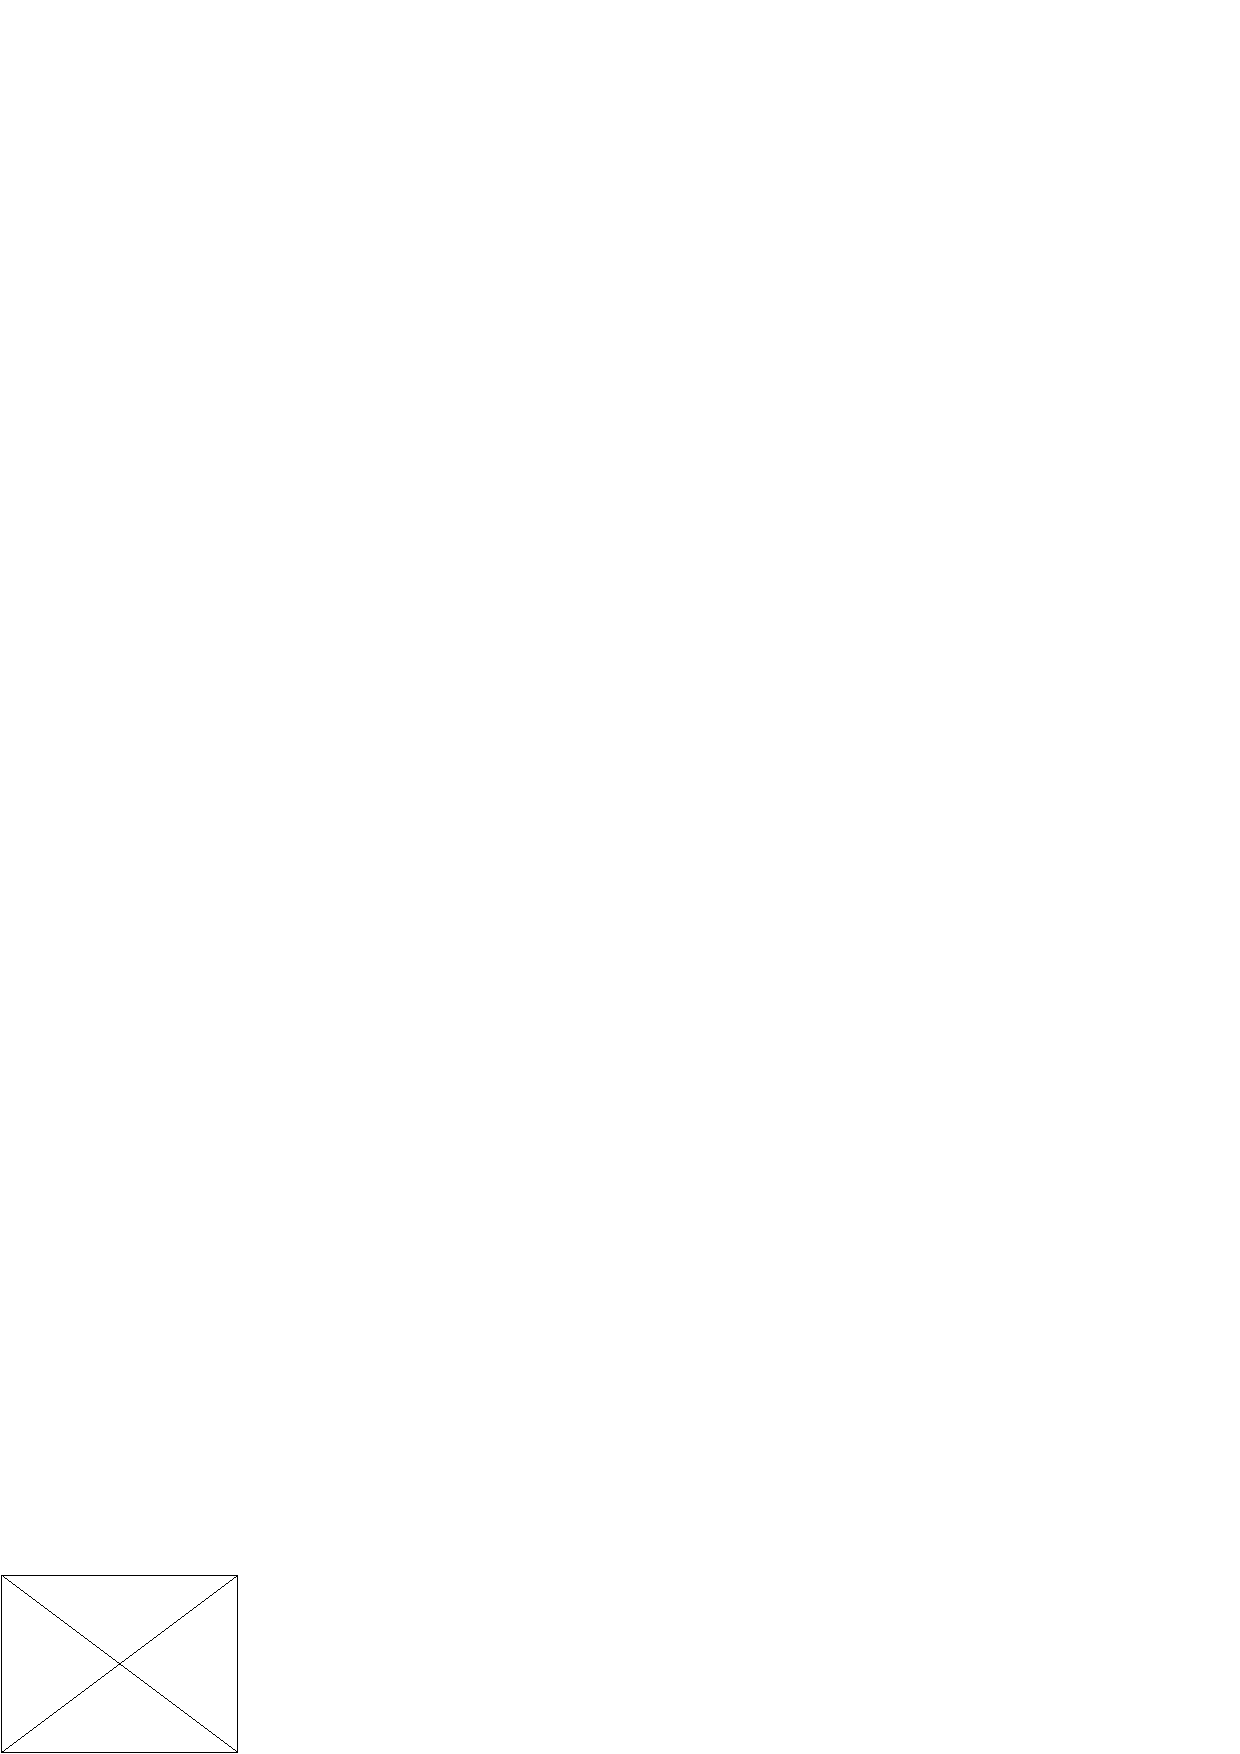
\includegraphics[height=10pc,width=78mm,draft]{empty}}
%\caption{This is an example for appendix figure.\label{fig5}}
%\end{figure}


\nocite{*}% Show all bib entries - both cited and uncited; comment this line to view only cited bib entries;
\bibliography{Biblio}%

\clearpage

\section*{Author Biography}

\begin{biography}{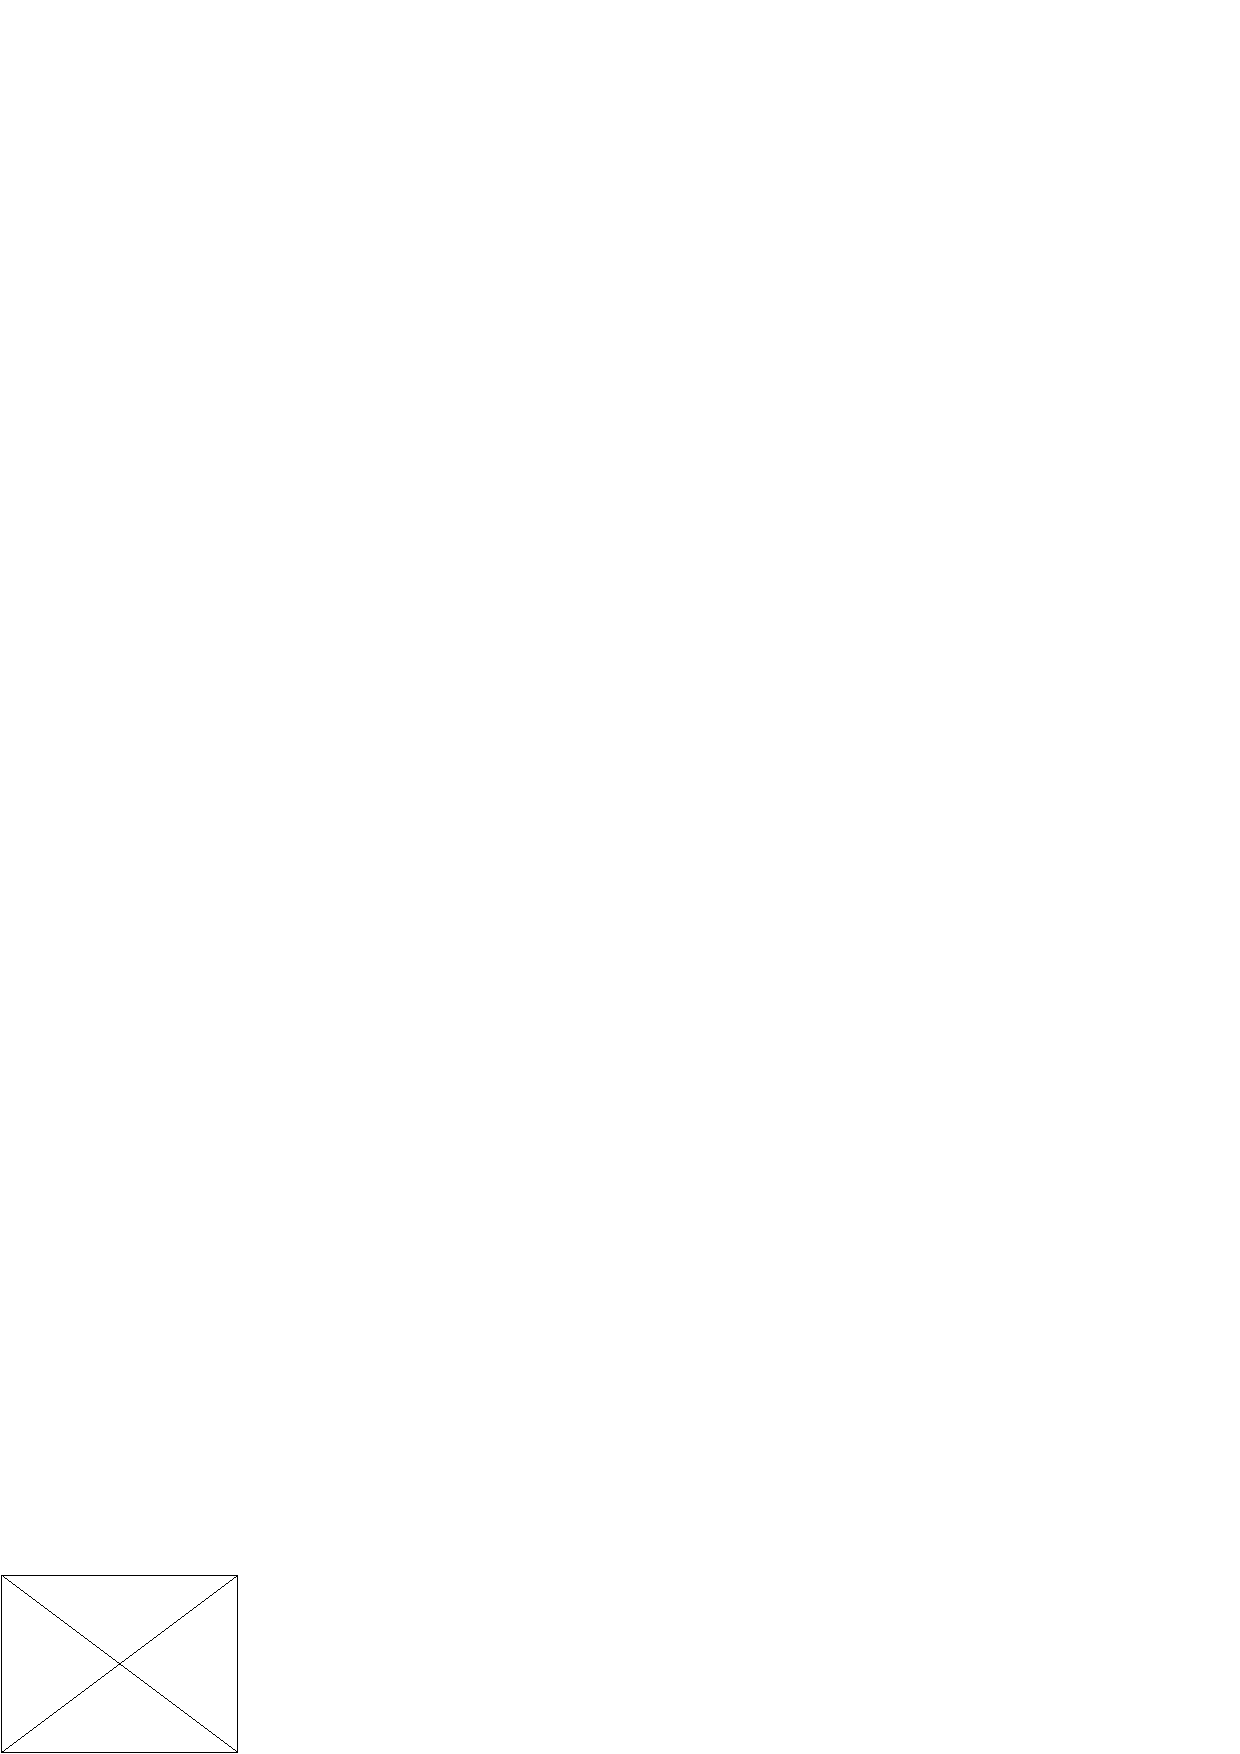
\includegraphics[width=66pt,height=86pt,draft]{empty}}{\textbf{Author Name.} This is sample author biography text this is sample author biography text this is sample author biography text this is sample author biography text this is sample author biography text this is sample author biography text this is sample author biography text this is sample author biography text this is sample author biography text this is sample author biography text this is sample author biography text this is sample author biography text this is sample author biography text this is sample author biography text this is sample author biography text this is sample author biography text this is sample author biography text this is sample author biography text this is sample author biography text this is sample author biography text this is sample author biography text.}
\end{biography}

\end{document}
